% https://tex.stackexchange.com/a/397008
\documentclass{beamer}


\usepackage{tikz}
\begin{document}

\begin{frame}
(....)
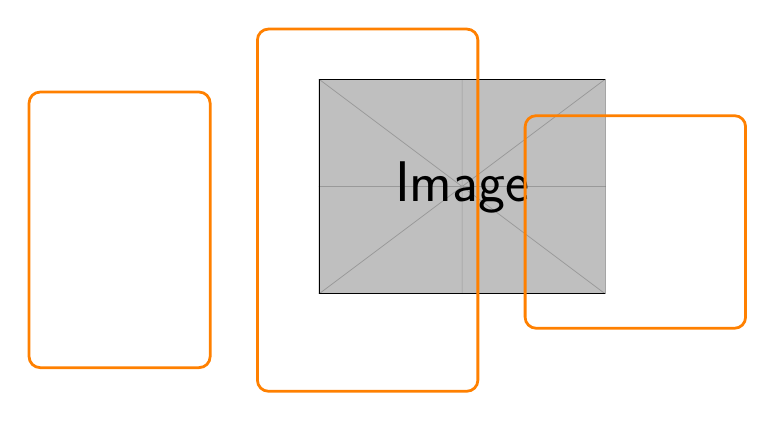
\begin{tikzpicture}
   \node (schematic) {\includegraphics[width=.3\textwidth]{example-image}};
   \pause
   \draw[orange,line width=1pt,rounded corners] (-5.5,-2.3) rectangle (-3.2,1.2);
   \pause
   \draw[orange,line width=1pt,rounded corners] (-2.6,-2.6) rectangle (0.2,2.0);
   \pause
   \draw[orange,line width=1pt,rounded corners] (0.8,-1.8) rectangle (3.6,0.9);
\end{tikzpicture}
\begin{itemize}
%   \pause
   \item<2-> \textbf{Box 1}: description 1;
%   \pause
   \item<3-> \textbf{Box 2}: description 2;
%   \pause
   \item<4-> \textbf{Box 3}: description 3;
\end{itemize}
(....)

\end{frame} 

\end{document}
